\documentclass[a4paper,12pt]{article}

\RequirePackage{epsfig}

\setlength\hoffset{-0.5in}      %% these work quite well with a 12pt font
\setlength\voffset{-0.5in}
\setlength{\textwidth}{6.30in}
\setlength{\textheight}{9.0in}

\bibliographystyle{unsrt}

\begin{document}

\begin{center}
{\Large\bf{Towards Evaluating Creativity in Language}} \\
      \vspace{5.0mm}
{\Large\bf{Project Plan}} \\
      \vspace{8mm}
      {\large\bf{Matey Krastev}}  \\
      \vspace{5.0mm}
       {\tt m.krastev.19@abdn.ac.uk} \\
      \vspace{5.0mm}
      {\em Department of Computing Science,\\
       University of Aberdeen, Aberdeen AB24 3UE, UK} 
\end{center}


\section*{Introduction}
The impact of large language models (LLMs) in recent years cannot be understated. 
Language models are finding their way in nearly every task imaginable, thanks to incremental improvements in the quality of prompt answers, suggestions and code tips. Some people even tend to use prompt-based models to answer their specific questions, in a way akin to how search engines operated in recent years. 

A model assisting workers in high-level abstraction jobs, such as those in creative writing, code development, medical practice and what are generally fields which require deep expertise in a variety of topics and enormous knowledge bases, can potentially spark a productivity boom similar to the ones experienced during the invention of semiconductors.

Most current language models, therefore, are trained on massive datasets comprising data almost on the order of magnitude of all resources available on the world wide web. Some would argue [[maybe insert ref]] that this would prove more than enough to satisfy the needs of the everyday consumer. However, defining one such LLM as artificial intelligence would largely neglect one of the most essential factors of human intelligence - creativity. 

Evaluating and benchmarking creativity is a task that has already been undertaken by researchers [[insert ref]] with varying degrees of success owing to the very abstract definition of the term itself. This project, therefore, seeks to compile and produce a software package that can efficiently, and more importantly, accurately represent creativity in language, or more formally, linguistic creativity. 

\section*{Goals}

As outlined above, we seek to answer two key questions. The first and most important being:

\begin{itemize}
    \item Can psycho-linguistically motivated measures (that is, the explored metrics) successfully characterise creative properties in language?
\end{itemize}
// does this give the evaluator confidence in the project?

And, following the successful implementation of the first, we shall attempt to answer the second question:
\begin{itemize}
    \item To what extent does hyperparameter tuning or varying decoding strategies on a given set of LLMs influence creativity as measured by our creativity metric?
\end{itemize}

To these ends, we develop a suite of benchmarks we shall distribute and report the results of.

% In other words, describe \emph{wht} it is that you want to do.
% Are you building a tool or an application? What functionality 
% already exists, and what will you have to do yourself?

% Try to make it clear which goals are central to your project, and which
% might be optional extras. Try to be realistic about making your
% goals {\em achievable.}


\section*{Methodology}
A major part of the project will be spent on research and iterative development of the benchmarks. This is a process that requires analysing and compiling resources on creative aspects of writing and language overall. Another major factor may be the development time spent on measuring the creativity of existing language models. A big chunk of contemporary language models based on neural networks, be those LSTM-, RNN-, or Transformer-based, can have a net size on the order of hundreds of millions of weights. These models need to be moved to a high-performance computing cluster, as even a high-end personal computer would not be able to handle having those in memory, let alone perform the number crunching. \newline A relatively high-level view of the development process would be:

\begin{itemize}
\item compiling and consulting available literature on the matter of creativity;
\item developing a systematic and rigorous set of benchmarks based on sound methods;
\item experimenting and finetuning the developed technology;
\item exploring potential exhibited creativity, prompted by hyperparameter tuning; 
\item larger-scale testing on HPC clusters and gathering result data;
\end{itemize}
%

\section*{Resources Required}
A mid- to high-end personal computer would be required for prototyping the metric, as well as building the interface and tools to interact with the system.  
Furthermore, a high-performance computing (HPC) cluster will be needed for utilising the large language models which have been open-sourced for research and general purposes. 
Python is the programming language of choice in the field of research and more specifically machine learning. It is a flexible language allowing the use of high-order abstractions interfacing with low-level fast, extremely CPU- and GPU-efficient operations. Therefore,  the development will be primarily carried out in Python via an interactive shell so that the system can be rapidly prototyped and improved upon. 

\section*{Risk Assessment}

The only major risks that threaten the successful execution of the project are schedule-based. The project is intensive and requires thorough research and dedication. Currently, we have mitigated this risk by carefully considering a schedule and goals outlined week by week. The schedule takes into account the authors' capabilities and seeks to not place a heavy burden on them during the project execution.

Frequent meetings with the project supervisor serve to check on the progress achieved in the past week, as well as to clarify the deliverables for the upcoming one. Through strict adherence to the timetable outlined below, we minimise the risks against the successful execution of the project.  

\section*{Timetable}
Please refer to Figure~\ref{fig:plan} outlined below. 

\begin{figure}[htb]
\begin{center}
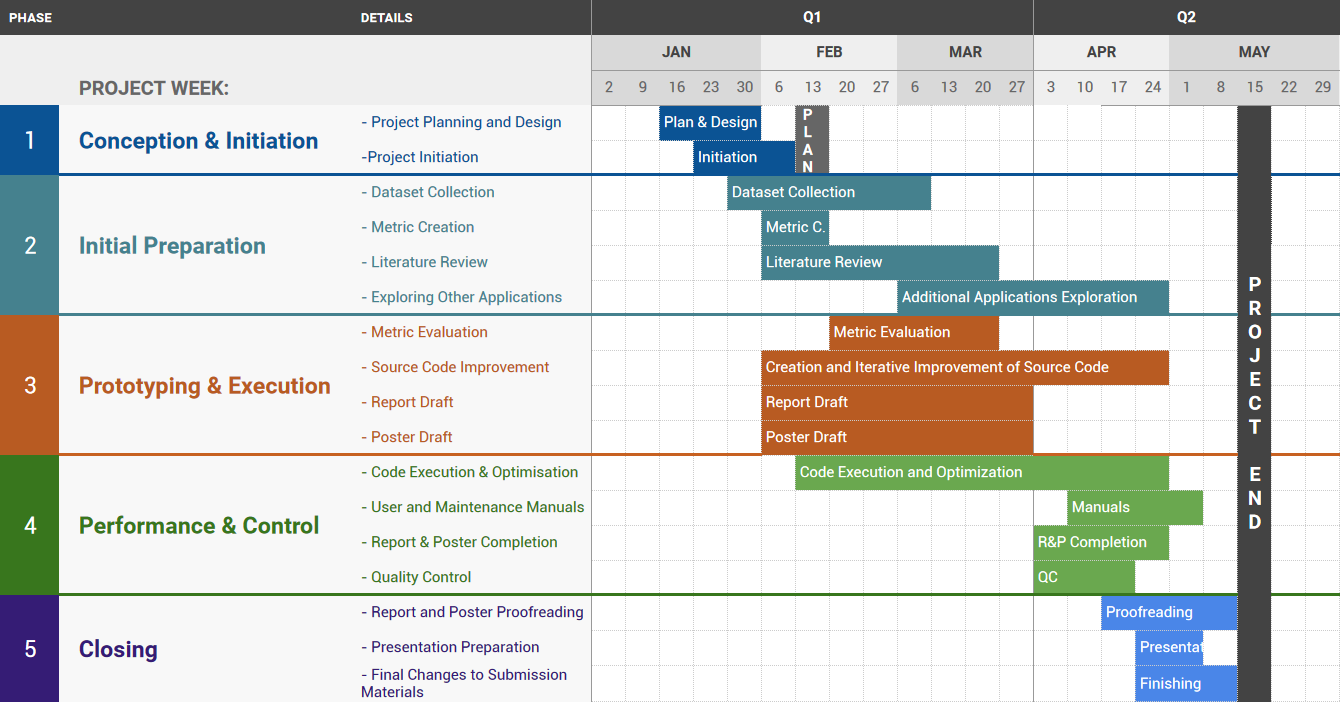
\includegraphics[width=\textwidth]{plan.png}
\caption{Main Project Activities \label{fig:plan}}
\end{center}
\end{figure}

% For information, this figure was created using xfig, and 
% converted to encapsulated postscript by a command in the Makefile
% before being included as a graphic in the \LaTeX document.

\bibliography{ProjectPlan}

\end{document}
